\documentclass[a4paper]{article}

\setcounter{secnumdepth}{0}

%Metadata
\title{Kuwaiba Open Inventory User's Manual}
\author{Neotropic SAS}
\date{27.07.2016}

%Imports
\usepackage{graphicx}
\usepackage[utf8]{inputenc}
\usepackage{booktabs}
\usepackage[margin=3cm]{geometry}
\usepackage{color}
\usepackage{framed}
\usepackage{verbatimbox}
\usepackage[toc,page]{appendix}
\usepackage{nameref}

%\usepackage{hyperref}

%Modify some defaults
\setlength{\parindent}{0pt} %don't indent new paragraphs

\begin{document}
	\maketitle
	\pagenumbering{gobble}
	
	
	
	\begin{figure}[b]
		\centering System Version \textbf{1.0}
			
		Visit \textbf{kuwaiba.org} for documentation, latest updates and upcoming events
	\end{figure}
	
	
	\newpage
	
	\tableofcontents

	\newpage
	\section{Document History}
		\begin{table}[h!]
			\centering
			\begin{tabular}{l||p{10cm}} %Each letter tells the parser what alignment should have every column
				\toprule
				\textbf{Date} & \textbf{Comments}  \\
				\midrule
				September 28th 2010 & First issue shipped with version 0.1.1\\
				\midrule
				November 26th 2010 & Update to cover the new features in 0.2 \\
				\midrule
				December 26th 2010 & Update to cover the new features in 0.2.1 \\
				\midrule
				January 18 th 2001 & Changes in version 0.3 alpha \\
				\midrule
				February 3 rd 2011 & Changes in version 0.3 beta \\
				\midrule
				March 13 th	2011 & Changes in version 0.3 beta 2 \\
				\midrule
				May 16th 2011 & Changes in version 0.3 stable (the clear button in the graphical query editor \\
				\midrule
				May 23rd 2012 & Adapted to version 0.4 \\
				\midrule
				October 23rd 2012 & Adapted to version 0.5 \\
				\midrule
				June 4 th 2013 & Added documentation	for Pools module \\
				\midrule
				June 12 th 2013 & Added documentation for Data model Manager module and some other minor changes\\
				\midrule
				January 19 th 2015 & Adapted manual for version 0.7 \\
				\midrule
				November 6 th 2015 & Added documentation about bulk upload, software asset management and detailed physical connections \\
				\midrule
				July 27th 2016 & Adapted to Kuwaiba version 1.0. LaTeX is now used instead of LibreOffice to create the documentation. \\
				\bottomrule
			\end{tabular}	
				
		\end{table}
	\newpage
	\section{License}
		\begin{table}[ht]
			\centering
			\begin{tabular}{cp{10cm}}
				
				
\includegraphics[]{img/cc_license_logo.jpg} & This document is published under the terms of a license Creative Commons by-nc-sa. You can find details about it at\linebreak
				\textbf{http://creativecommons.org/licenses/by-nc-sa/2.0/ } \\

				
\includegraphics[width=2cm]{img/osi_logo.jpg} & Kuwaiba Server and Client are licensed under EPL v1 and GPL v2. You can find the whole text of this licenses at \linebreak
				\textbf{http://www.eclipse.org/legal/epl-v10.html} \linebreak
				\textbf{http://www.gnu.org/licenses/old-licenses/gpl-2.0.html} \\
			\end{tabular}
		\end{table}
		\paragraph{Disclaimer} \hspace{0pt}
		\begin{itemize}
			\item Netbeans and Java are registered trademarks of Oracle and/or its affiliates. Other names may be trademarks of their respective owners. The Kuwaiba project is not endorsed to any of them.
			
			\item This document is provided “as is”, with no warranty at all. Install the software and follow the instructions included at your own risk.
			
			\item Kuwaiba uses third-party components with compatible open source licenses (LGPL, BSD-like, etc). You can find a complete list at the project's web page.
		\end{itemize}
	
	\newpage
	\pagenumbering{arabic}
	\section{Introduction}
	Kuwaiba sees an inventory system as a living entity, not growing only in terms of size, but also in structure and intelligence. The main reason is that business requirements change constantly and therefore, the application must ready to respond to new scenarios. One of the key concepts that can help you unlock the potential of Kuwaiba is the \textbf{data model}. It provides a simplified representation of the network and the business from an operational point of view. It can be seen as the skeleton that supports the application, but a skeleton from which you can add, remove and change elements as you go. Later in this document you will be able to see what tools you can use to manage it. For now, just keep in mind that the better you design your data model and the more you get to know it, the more you will take advantage of the application.\newline
	
	Having said that, you will find four types of resources in a typical data model:
	\begin{itemize}
		\item \textbf{Physical:} Equipment, pipes, cables, fiber optics, facilities, parts and in general every physical asset from a port to a building. 
		\item \textbf{Logical:} These are all the resources related to non-tangible technology assets. In this group fits timeslots, virtual circuits, VLANs, disk space, available bandwidth, etc.
		\item \textbf{Other Non-physical:} mostly software-related assets, such as licenses or virtual machines.
		\item \textbf{Administrative:} These are all those related to administrative tasks, human resources or commercial management. Customers, their services, SLAs (and related parameters like availability or throughput), sales and technical staff assigned to those services, vendors and states belong to this category.
	\end{itemize}
	The Kuwaiba desktop client is a set of views (trees, topologies, editors) that allow to put together these elements based on business rules and  user-defined models. Kuwaiba extends the concept of \textbf{CMDB} (Configuration Management Database, a place where you store objects that can hold configuration information or be subject to configuration themselves -so called Configuration Items- and their relationships)  and enables you to perform network design tasks, support capacity management and provisioning workflows and assist field and customer service teams to improve response times.\newline
	
	Kuwaiba helps you model your network according to your needs, no matter if you're an ISP, a carrier or just a guy with a large (or small!) IT infrastructure to manage. It's open source, under active development and new models are added every release. You can contribute to the project by providing technical insight on a particular technology, testing, translating or just sending your feedback through forums\footnote{Forums https://sourceforge.net/p/kuwaiba/discussion/} and mailing lists\footnote{mailing lists https://sourceforge.net/p/kuwaiba/mailman/}.
	
	\newpage
	\section{Connection to the Server}
	The first thing you will see when opening the client is the window in the figure~\ref{fig:auth_window}. The default user and password are \textbf{admin/kuwaiba}.
	 
	\begin{figure}[h!]
		\centering
		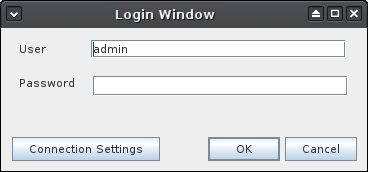
\includegraphics[width=0.5\linewidth]{img/auth_window.png}
		\caption{Authentication window}
		\label{fig:auth_window}
	\end{figure}
	The default connection settings should be enough if the server is running on the same computer the client is. If that's not the case, open the Connection Settings window (figure~\ref{fig:connection_settings}).
	\begin{figure}[h!]
		\centering
		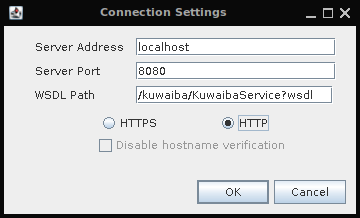
\includegraphics[width=0.5\linewidth]{img/connection_settings.png}
		\caption{Connection Settings window}
		\label{fig:connection_settings}
	\end{figure}
	\begin{itemize}
		\item \textbf{Server Address} Refers to the server IP address or canonical name.
		\item \textbf{Server Port} is the port Glassfish (the application server) is listening to.
		\item \textbf{WSDL Path} is the path within the application server the web service interface definition can be found. Usually this value should remain unchanged.
		\item Protocol is the transport protocol to be used. By default is HTTP, but is highly advisable to request your administrator to setup a secure connection, otherwise your credentials will be transmitted in plain text over the network. 
	\end{itemize}
	Except for the password, the last successful settings will be saved upon clicking OK.
	\begin{framed} {\large \textbf{Important}} \\
		If you are unsure if the server is reachable from your location, open a browser and type the address: \textbf{http://[server\_address]:[server\_port]/[wsdl\_location]}\\
		
		You should see a large XML document.
	\end{framed}
	\begin{framed} {\large \textbf{Troubleshooting}}
		\begin{itemize}
			\item For a \textbf{\textcolor{red}{Can't contact backend}} error, check the Administrator's Manual Troubleshooting section.
			\item If you get a \textbf{\textcolor{red}{Connection refused}} error, check the connection settings and verify that the server is reachable and there isn't a firewall blocking the traffic to it.
		\end{itemize}
	\end{framed} 
	Once you are logged in, you will see only the dashboard page and a toolbar (figure~\ref{fig:main_toolbar}).\\
	\begin{figure}[h!]
		\centering
		
\includegraphics[width=0.7\linewidth]{img/main_toolbar.png}
		\caption{Main toolbar}
		\label{fig:main_toolbar}
	\end{figure}
	
	The toolbar contains the most frequently used tools. Here is an overview of what cab you do with them:
	\begin{table}[h!]
		\centering
		\begin{tabular}{cl}
			
\includegraphics[width=0.5cm]{img/icon_query_manager.png} & Search objects with the Query Manager\\
			\midrule
			
\includegraphics[width=0.5cm]{img/icon_refresh_component.png} & Refresh the current view\\
			\midrule
			
\includegraphics[width=0.5cm]{img/icon_refresh_cache.png} & Refresh local cache\\
			\midrule
			
\includegraphics[width=0.5cm]{img/icon_object_view.png} & Default view for an object. Also, the rack view for rack objects\\
			\midrule
			
\includegraphics[width=0.5cm]{img/icon_task_manager.png} & Create automation tasks (beta version)\\
			\midrule
			
\includegraphics[width=0.5cm]{img/icon_audit_trail.png} & See the changes made to inventory and application objects\\
			\midrule
			
\includegraphics[width=0.5cm]{img/icon_user_manager.png} & Manage users and groups\\
			\midrule
			
\includegraphics[width=0.5cm]{img/icon_data_model_manager.png} & Change the data model\\
			\midrule
			
\includegraphics[width=0.5cm]{img/icon_containment_manager.png} & Manage how objects can be created inside others\\
			\midrule
			
\includegraphics[width=0.5cm]{img/icon_list_type_manager.png} & Create new list types\\
			\midrule
			
\includegraphics[width=0.5cm]{img/icon_topology_designer.png} & Freely design network topologies\\
			\midrule
			
\includegraphics[width=0.5cm]{img/icon_navigation_tree.png} & Main tree used to explore physical assets\\
			\midrule
			
\includegraphics[width=0.5cm]{img/icon_pools_manager.png} & Create and manage objects that don't fit in the navigation tree\\
			\midrule
			
\includegraphics[width=0.5cm]{img/icon_service_manager.png} & Manage client, services and resources associated to them\\
		\end{tabular}	
		\caption{Toolbar items}
		\label{tab:toolbar_icons}
	\end{table}
	
	\newpage
	\section{Data Model Manager} \label{sec:data_model_manager}
		One of the key features of Kuwaiba is that it is completely object-oriented\footnote{Object-oriented Programming https://en.wikipedia.org/wiki/Object-oriented\_programming}. It means that every business (Router, City, Port) and application (users, types) element is represented by an \textbf{Object} in the application and these objects are in turn product of an reality abstraction called \textbf{Class}. Likewise, every attribute is a \textbf{Field} in a class. The set of classes, attributes and relationships between them is called data model. There's a default data model, but you can customize it depending on your needs by adding, removing and modifying classes. To achieve this, use the Data Model Manager module (figure~\ref{fig:data_model_manager}).
		\begin{figure}[h!]
			\centering
			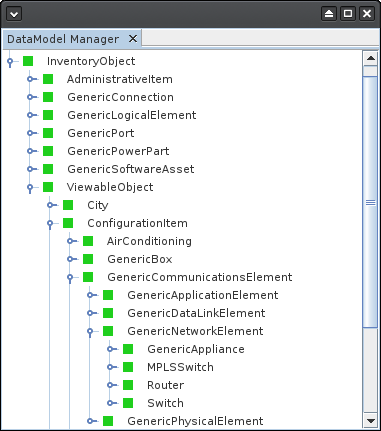
\includegraphics[width=0.4\linewidth]{img/data_model_manager.png}
			\caption{Part of the data model tree}
			\label{fig:data_model_manager}
		\end{figure}
		The data model is represented as a tree because it's a hierarchical structure. Technically, it's a class hierarchy\footnote{Class Hierarchy https://en.wikipedia.org/wiki/Class\_hierarchy}. The top of the hierarchy (\textbf{InventoryObject}) is the most general type of element in the data model and its subclasses represent all the possible elements that will be treated as inventory assets. As you dig deeper into the tree, the classes become more and more specialized and each level inherits the attributes of the parent classes. This kind of structure has two purposes: First, it helps you to organize your classes based on what characteristics they have in common. Secondly, as you will see later in this manual, you can apply operations over top level classes, and they will be propagated to all subclasses. Another root of the data model tree is \textbf{GenericObjectList}, and its subclasses are all possible list types (see more details on the subject in the chapter \textbf{\nameref{sec:list_type_manager}}).\newline
		
		\begin{framed} {\large \textbf{Important}} \\
				The \textbf{Properties} window allows you to modify the attributes of a selected object in a tree, list or view. If not already open, it's available from the Windows $\rightarrow$ Properties menu.
		\end{framed}
		The properties of a class can be edited by using the \textbf{Properties} window, selecting the class from the tree (see figure~\ref{fig:properties_class_node}). 
		\begin{figure}[h!]
			\centering
			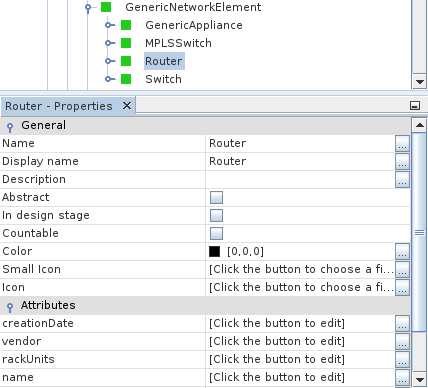
\includegraphics[width=0.5\linewidth]{img/properties_class_node.png}
			\caption{Properties of class \textbf{Router}}
			\label{fig:properties_class_node}
		\end{figure}
		The  property  sheet  is  divided  in  two  sections: 
		\begin{itemize}
			\item \textbf{General:} Contains the intrinsic properties  of  the class: \textbf{name} (can contain only letters and numbers with no special characters  or  blank  spaces). The  \textbf{display name} of the class, that's how the  will be displayed everywhere else (useful  for  internationalization  purposes, for example) and can contain any kind of UTF-8 character. A \textbf{description} (useful  to  document  the  data  model). If  the class is \textbf{abstract} (abstract classes  cannot  be  instantiated, they're only used to give consistency to the  data  model). The attribute \textbf{countable} is not used currently, but it should be used to mark classes whose instances can have graphical representations, but  they're  not really  part  of  the  inventory,  such  as  \textbf{Slots}. \textbf{In Design Stage} is just a way to mark a class as part of an ongoing data model intervention, and thus, classes with that attribute set to true can not be instantiated. \textbf{Color} is the color of the default square icon used to display the object in a tree or view. This icon will be used as long as the \textbf{Small Icon} attribute is null. \textbf{Small Icon} is the icon that will be used in trees and its size can't exceed 16x16 pixels. \textbf{Icon} is the icon used in views, and has a maximum size of 32x32 pixels.
			\begin{framed} {\large \textbf{Important}}
				\begin{itemize}
					\item All user-created classes are set In Design Stage = \textbf{\textcolor{green}{true}} by default. You won't be able to create objects of these classes until you set it to \textbf{\textcolor{blue}{false}}.
					\item As a convention, all abstract classes have the prefix \textbf{Generic}. Note that a few core classes (like \textbf{InventoryObject} or \textbf{\textcolor{green}{true}}) are abstract are the exception to this rule. You, however, should try to follow this convention as much as possible.
				\end{itemize}
			\end{framed}
			\item The second section  contains the class fields (attributes). In the  figure\ref{fig:properties_class_node}, class Router  has six attributes: name, state, conditions, vendor, serialNumber and creationDate. Click the button next to the attribute name to customize it (see figure~\ref{fig:class_attribute_details}).
			\begin{figure}[h!]
				\centering
				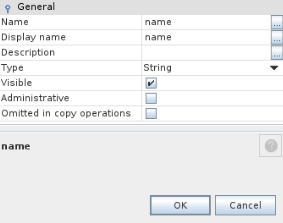
\includegraphics[width=0.4\linewidth]{img/class_attribute_details.png}
				\caption{Properties of attribute \textbf{name} in class \textbf{Router}}
				\label{fig:class_attribute_details}
			\end{figure}
		\end{itemize}
		In this window, you can modify the attribute's name, display name, description, type  (the drop-down list will show you primitive types -String, Integer, Float, Long, etc- and all available non-abstract list types). When you change an attribute's type, all existing instances will be	modified to reflect the change, which means that the values of the modified attribute will be converted to the new type if possible (say, from Integers to Strings). If the conversion is not possible, the new value will be set to null. You  can  also  manage  the  attribute  visibility. Attributes marked as “Administrative” will be shown in a separate tab in the object's property sheet. Sometimes, there are  attributes that are used only for administrative purposes and might confuse the end user if mixed with the regular attributes. Finally, you can choose what attributes shouldn't be transferred from one object to another in a copy operation.
		
		\begin{framed} {\large \textbf{Important}}
			\begin{itemize}
				\item You may lose information when changing an attribute's type. make sure the conversion to the new type is possible before you do it.
				\item Although there's a Cancel button at the bottom of the window, it does not	really work. When you perform a change, it's saved immediately.
			\end{itemize}
		\end{framed}
		You can also create and delete classes and attributes by right-clicking a class node (see figure~\ref{fig:class_node_menu})
		\begin{figure}[h!]
			\centering
			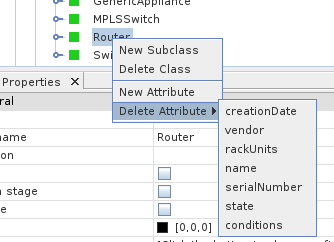
\includegraphics[width=0.4\linewidth]{img/class_node_menu.png}
			\caption{Class \textbf{Router} context menu}
			\label{fig:class_node_menu}
		\end{figure}
		New subclasses inherit the parent class attributes. Classes with instances or subclasses can not be deleted (this is  a  feature to avoid unintended loss of  data). Also, attribute \textbf{name} can not be deleted.
		\begin{framed} {\large \textbf{Important}}
			It's highly recommended \textbf{\textcolor{red}{NOT}} to rename abstract core classes, as some of them are used internally to support many features and renaming them may turn the system unstable.
		\end{framed}
		
	\newpage
	\section{Containment Manager} \label{sec:containment_manager}
	Another key concept in Kuwaiba is containment. It consists of the ability to define what kind of objects can be created within others. For example, a \textbf{Country} can be inside a \textbf{Continent}, but can't be inside a \textbf{Rack}. A \textbf{Port} is usually within a \textbf{Board}, and not inside a \textbf{City}. These business rules can be defined using the Containment Manager.
	
	\begin{figure}[h!]
		\centering
		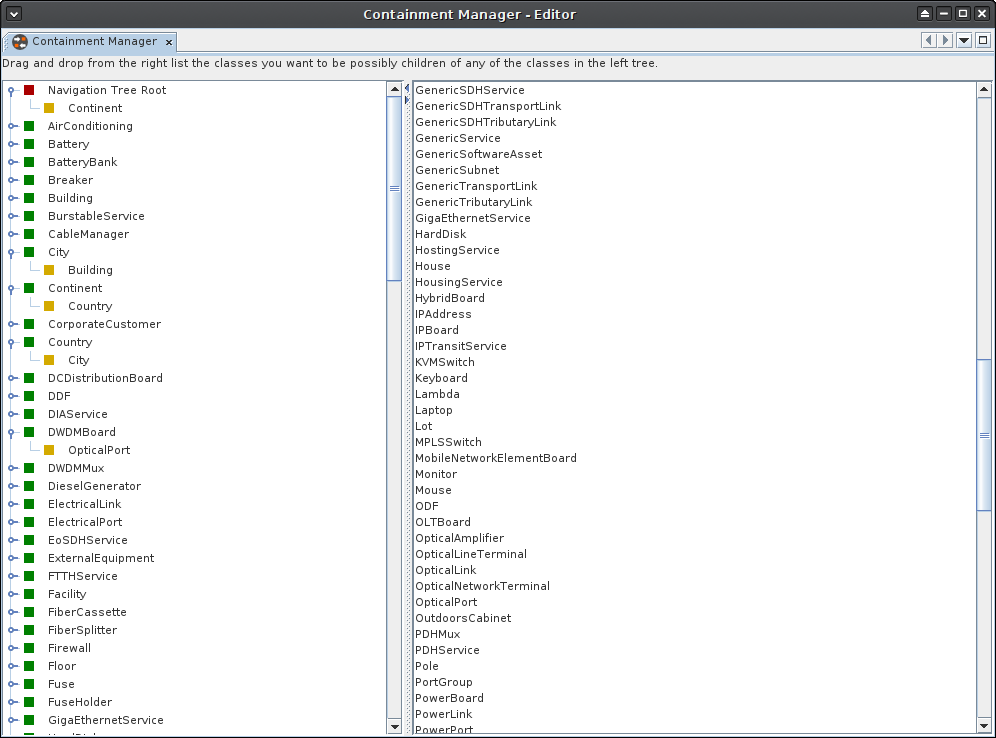
\includegraphics[width=0.7\linewidth]{img/containment_manager.png}
		\caption{Containment Manager main window. Zoom in the image to see the details}
		\label{fig:containment_manager}
	\end{figure}
	The main window is divided in two panels (see figure~\ref{fig:containment_manager}, zoom in the image to see the details). The one on the left is a tree that holds all the classes plus the \textbf{Navigation Tree Root}. The children of the left-side tree node are the possible classes that can be contained. In the figure~\ref{fig:containment_manager} there are five nodes expanded: \textbf{City}, that has one node inside: \textbf{Building}. That means that below a given city, you will only be able to add \textbf{Building} objects. Likewise, inside a \textbf{Continent} you can only create instances of \textbf{Country}, and inside those instances, only objects of class \textbf{City}. Under the root of the Navigation Tree, only instances of \textbf{Continent} are to be created. Finally, only \textbf{OpticalPorts} are supported under \textbf{DWDMBoards}. If for your operation Continents are not relevant, or if your routers do not have boards, but only ports, simplify the hierarchy as much as you want to meet your needs. To remove a possible children class, just right-click on it and select “Remove”, and instances from that class will no longer be available to be added under the parent class, though the objects created already will remain linked to the respective parent objects.
	\begin{framed} {\large \textbf{Important}}
		\begin{itemize}
			\item To avoid adding one by one many classes to a parent, you can use the flexibility of the data model as a hierarchical structure. For example, a \textbf{Rack} may contain within many types of equipment (routers, DDFs, switches, battery banks, etc). Instead of adding one by one each of these classes, you can add a common super class and all of them will be added automatically. For this example a common super class for most of those classes could be \textbf{GenericCommunicationsElement}.
			\item To search for a particular class, just select any node in the desired side of the panel and type the first letters of the class name. If there are many occurrences of the term, jump from one to another using the F3 key.
			\item The changes are applied immediately, however, if you happen to not see them reflected, press the Refresh Cache button in the main toolbar (see table~\ref{tab:toolbar_icons}).
		\end{itemize}
	\end{framed}
	\newpage
	
	\newpage
	\section{Navigation Tree} \label{sec:navigation_tree}
	This module presents in a tree fashion the physical objects of your inventory organized according to the containment hierarchy defined with the tool described in the previous chapter (see \textbf{\nameref{sec:containment_manager}}).
	\begin{figure}[h!]
		\centering
		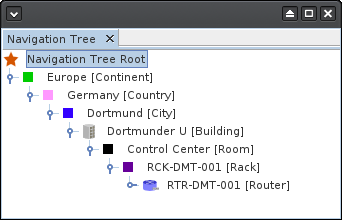
\includegraphics[width=0.4\linewidth]{img/navigation_tree.png}
		\caption{Navigation tree showing objects with default and user-defined icons}
		\label{fig:navigation_tree}
	\end{figure}
	Just like the \nameref{sec:data_model_manager}, the Properties window will display the attributes of the object selected in the Navigation Tree. These attributes match the visible attributes defined in the \textbf{\nameref{sec:containment_manager}}.
	\begin{figure}[h!]
		\centering
		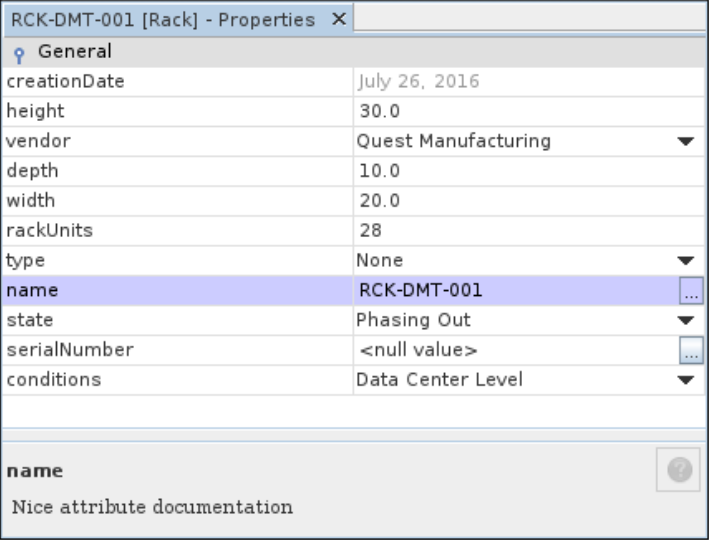
\includegraphics[width=0.5\linewidth]{img/navigation_tree_properties.png}
		\caption{Properties of a selected \textbf{Rack} object}
		\label{fig:navigation_tree_properties}
	\end{figure}
	Every change is automatically committed to the database once you hit the Enter key. When editing dates, you need to select another attribute to commit the changes instead of pressing Enter. In the \textbf{\nameref{sec:containment_manager}} you can also configure what labels will be displayed instead of the actual names of the attributes and the help string in the lowest part of the window.\newline
	
	Every node has a set of actions, some will be active for all objects, some depend on the type of element that is selected. In the figure~\ref{fig:navigation_tree_context_menu} you can see the actions enabled for a \textbf{Rack} object. \\
	\begin{figure}[h!]
		\centering
		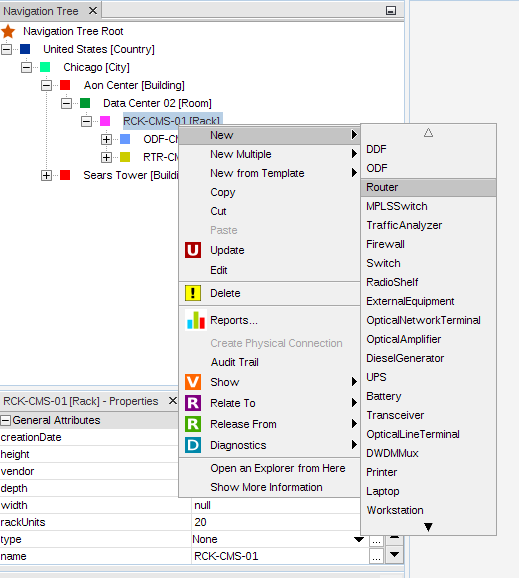
\includegraphics[width=0.5\linewidth]{img/navigation_tree_context_menu.png}
		\caption{Properties of a selected \textbf{Rack} object}
		\label{fig:navigation_tree_context_menu}
	\end{figure}
	\begin{itemize}
		\item \textbf{New Object:} The list of object types that can be contained for the selected element type according to the configured Containment Hierarchy. In this case, a \textbf{Rack} can only contain \textbf{Routers}.
		\item \textbf{Copy:} A plain copy operation.
		\item \textbf{Paste:} A plain paste operation. You can only paste objects where it is allowed according to the configured Containment Hierarchy.
		\item \textbf{Update:} Update the node information. Useful when a changed has made to the object from a external source (e.g. another user) or if you create a new list type affecting one of the attributes of the selected element. In this case, if you, for example, create an instance of \textbf{EquipmentVendor} (this will add a new entry to the \textbf{vendor} attribute list)
		\item \textbf{Delete:} Deletes the object. Tis will fail if the object has an incoming relationship, for example, a \textbf{Port} connected to a cable.
		\item \textbf{Reports:} The reports associate with this class. In this case, \textbf{Rack} has a report called \textbf{Rack Usage}. If no reports are associated, the option will appear grayed out.
		\item \textbf{Relate to service:} All inventory objects can be associated to an existing service. See more details in the chapter \nameref{sec:service_manager}.
		\item \textbf{Release from Service:} Removes the association between an object(resource) and a service. If the object is not related to any service, this option will appear grayed out.
		\item \textbf{Audit Trail:} This will display all the audit trail entries for the selected object, that is, all the changes made to the it.
		\item \textbf{Open an Explorer from this Node:} Opens a navigation tree whose root node will be the selected object. Useful when you want to explore an object with a many containment levels below.
		\item \textbf{Show Object Id:} Shows the database id of the selected object. Useful for troubleshooting purposes. It will also show the object's complete containment structure.
			\begin{figure}[h!]
				\centering
				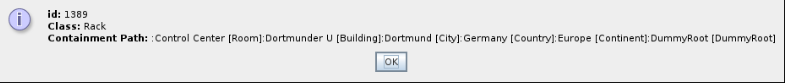
\includegraphics[width=\linewidth]{img/action_show_object_id.png}
				\caption{Object id action on the selected \textbf{Rack} object}
				\label{fig:action_show_object_id}
			\end{figure}
	\end{itemize}
	\begin{framed} {\large \textbf{Important}}
		\begin{itemize}
			\item Remember that you can always open the Properties window by selecting the main menu option Windows $\rightarrow$ Properties.
			\item You can change the name of an object in-line by pressing F2 on a selected node.
		\end{itemize}
	\end{framed}
	\subsection{Relationship and Special Children Explorer} \label{sec:extra_explorers}
	Apart from the main navigation tree, there are also two explorers that are very useful to navigate through domain-specific models. Both explorers are located in the Tools $\rightarrow$ Navigation menu.
	\begin{itemize}
		\item \textbf{Relationship Explorer:} Allows to see the special relationships of the selected object. When an object makes part of a domain-specific model (SDH, Physical Connections, MPLS, Software Licensing, etc) there are special bounds to other objects called \textbf{relationships} they have names documented on model-basis, and they can be seen using this explorer. In the figure~\ref{fig:navigation_tree_relationship_explorer}, it is depicted an \textbf{OpticalPort} with two relationships, one called \textbf{endpointA} used in the Physical Connections model and it indicates that this port is the endpoint to a physical connection, probably a fiber optic. It also has a relationship called \textbf{uses}, which makes part of the Service management model. It indicates that the service called PDH Service-01 uses that port as a resource.
			\begin{figure}[h!]
				\centering
				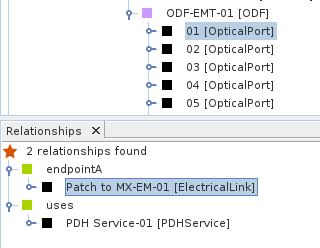
\includegraphics[width=0.4\linewidth]{img/navigation_tree_relationship_explorer.png}
				\caption{Special relationships of the selected \textbf{OpticalPort} object}
				\label{fig:navigation_tree_relationship_explorer}
			\end{figure}
		\item \textbf{Special Children Explorer:} The special children are children as in the containment hierarchy concept, but used in domain-specific models, which gives them particular behavior depending on the situation (that is, they can't be handled as simple objects in the navigation tree, because, for example, deleting them may require to perform other tasks but just removing the object from the database as they make part of a complex workflow). This is the case of the cables inside a conduit connecting two buildings. You can find more details about this scenario in the chapter \textbf{\nameref{sec:physical_connections}}.
			\begin{figure}[h!]
				\centering
				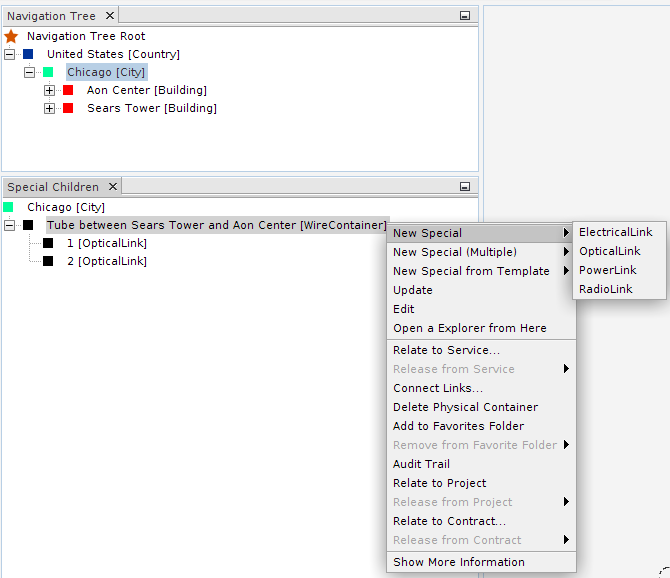
\includegraphics[width=0.3\linewidth]{img/navigation_tree_special_children_explorer.png}
				\caption{Fibers inside a container between two buildings}
				\label{fig:navigation_tree_special_children_explorer}
			\end{figure}
	\end{itemize}
	
	\newpage
	\section{Physical Connections} \label{sec:physical_connections}
	
	\newpage
	\section{List Type Manager} \label{sec:list_type_manager}
	
	\newpage
	\section{Audit Trail} \label{sec:audit_trail}
	
	\newpage
	\section{Service Manager} \label{sec:service_manager}
\end{document}